\documentclass[a4paper,12pt]{article}

\title{Programmering og Problemløsning, ugeseddel 1}
\author{Version 1.5}% Torben Mogensen, Hans Jacob Teglbjærg Stephensen
\date{14.\ marts 2015}

\usepackage[top=2cm,left=25mm]{geometry}
\usepackage[T1]{fontenc}
\usepackage[utf8]{inputenc}
\usepackage[danish]{babel}
%\usepackage{microtype}
\hyphenpenalty=750

\usepackage{amsmath}
%\usepackage{lmodern}
%\usepackage{mathptmx}
%\usepackage{libertine}
%\usepackage[scaled=0.90]{inconsolata}
%\usepackage[scaled=0.83]{beramono}

\usepackage{enumerate}
\usepackage{listing}
\usepackage{fancyvrb}
\usepackage{graphics,tikz}



\usepackage{hyperref}
\hypersetup{pdftitle={Introduktion til programmering, ugeseddel 1},
            pdfsubject={},
            pdfauthor={},
            pdfkeywords={SML, rekursion, funktioner},
            pdfborder={0 0 0}}

\setlength{\parskip}{1ex}
\setlength{\parindent}{0pt}
\setlength{\parfillskip}{30pt plus 1 fil}


\begin{document}
\maketitle{}

Velkommen til kurset ``Programmering og Problemløsning''.

Dette er den første af i alt~14 \emph{ugesedler}. Ugesedlerne
indeholder information om ugens opgaver samt diverse praktisk
information og perspektivering af ugens pensum.

Den første undervisningsuge har til formål at gøre dig fortrolig med
redigering og afvikling af programmer med Emacs og F\# Interactive fsi (fsharpi på linux).

\textbf{>>[Rework needed]} (ordvalg "perfekt", per email til instruktor?)\\
Der er ingen obligatoriske opgaver i uge 1, men der er stillet en
gruppeopgave og en individuel opgave som træning til de efterfølgende obligatoriske opgaver. Det anbefales stærkt, at aflevere begge opgaver. Der gives feedback til jeres afleveringer, som kan være nyttig til de senere opgaver.  Denne uges opgaver kan I aflevere så mange gange I lyster og få ny feedback, så I kan øve jer i at lave en perfekt aflevering.  Giv jeres instruktor besked (email) ved nye afleveringer.

Vi bruger følgende lærebøger:

\begin{itemize}
\item Hansen \& Rischel: \textit{Functional Programming Using F\#},
  Cambridge University Press 2013. Vi forkorter denne som ``HR''.
\end{itemize}

Vi antager at du allerede har anskaffet dig bøgerne ved kursusstart. De kan begge købes i Polyteknisk Boghandel i Biocenteret.


\section{Pensum og plan for ugen}
\label{sec:pensum-og-plan}

\textbf{>>[Rework needed]}\\
\textbf{Pensum for uge 1:} HR kap. 1 og 2, IP-2 kap. 1, 2 og 3 (1.7 dog kun kursorisk).

\textbf{Foreslået læserækkefølge:} IP-2, kap. 1, HR kap. 1 og 2, og dernæst
IP-2 kap. 2 og 3.

Forelæsningen mandag vil fokusere på at skrive simple udtryk og
funktioner i emacs og køre dem i F\# Interactive. Hyppigt forekomne
fejlmedelelser vil blive forklaret. Øvelserne vil give hjælp til
installering af Eduroam, Emacs og mosml til de studerende, der ikke
har gjort det allerede, og der vil derefter laves simple funktioner i
mosml.

Tirsdag omhandler både forelæsninger og øvelser rekursive
funktionserklæringer, par/tupler (sæt), betingede udtryk og simple
typer, herunder heltalsaritmetik.

Fredag introducerer tegn (\texttt{char}) og tekster
(\texttt{string}). Øvelserne bruges til at arbejde med den
individuelle opgave.


%\newpage
\section{Mandagsopgaver}
\label{sec:mandagsopgaver}

Mål: Fortrolighed med \texttt{mosml} systemet, heltal og kommatal,
sandhedsværdier, unære og binære operatorer og operatorpræcedens.

\begin{enumerate}[{1}M1]
\item Følg din instruktors anvisninger til installering af
  F\#, og Emacs på din bærbare. Hvis du ikke har en med selv, så kig
  med hos en anden.
\item Opsæt (med hjælp fra instruktor) Eduroam på din bærbare.
\item Log ind på KUnet og find Absalonsiden for PoP.
\item Start F\# Interactive.
\item \textbf{>>[Rework needed]} Evaluer udtrykkene \verb|2+3|, \verb|2.0+3.0| og \verb|2+3.0| i F\# Interactive husk at udtryk skal afsluttes med \verb|;;| og vigtigs, bemærk forskellene mellem resultaterne. Hvad skyldes de?
\item Evaluer udtrykket \verb|2-3|. Hvordan ser fortegnet på resultatet
  ud?
\item \textbf{>>[Discussion needed]} Evaluer udtrykkene \verb|-3 - -5| og \verb|-3 --5| (bemærk forskellen på
  mellemrumstegn). Hvad sker der?
\item Evaluer udtrykket \verb|9*9|, og gentag derefter evaluering af
  udtrykket \verb|it*it| fire gange. Hvad sker der, og hvorfor?
\item Evaluer udtrykket \verb|99.0 * 99.0|, og gentag derefter
  evaluering af udtrykket \verb|it*it| syv gange. Hvad sker der, og hvorfor?
\item Evaluer i mosml udtrykkene \verb|2<3|, \verb|2=3|, \verb|3<=3|, \verb|3>=3|, \verb|3>3| og \verb|4<>4|.
\item Evaluer udtrykkene \verb|2+3*4| og \verb|(2+3)*4|.  Forklar forskellen.
\item Evaluer udtrykkene \verb|2+3<4| og \verb|2+(3<4)|.  Forklar forskellen.
\item Skriv i Emacs en fil \texttt{plus5.fsx}, der indeholder en
  funktionserklæring til en funktion \verb|plus5|, sådan at funktionskaldet
  \verb|plus5(n)| evalueres til $n + 5$ for alle heltal $n$. F.eks. skal kaldet
  \verb|plus5(7)| evaluere til værdien \verb|12|. Hent funktionen ind i F\# Interactive med
  kommandoen \verb|#load "plus5.fsx";;|. Hvilken type har funktionen? Hvad
  sker der, når du laver kaldene \verb|plus5(7)|, \verb|plus5 7|, \verb|plus5(7.0)| og
  \verb|plus5("7")|?
\item \textbf{>>[Rework needed]} Hvis der er tid tilovers, så regn opgave 2.1--2.9 i IP-2.
\end{enumerate}

\newpage
\section{Tirsdagsopgaver}
\label{sec:tirsdagsopgaver}

Mål: Læse, håndkøre og skrive simple rekursive funktioner.

Det forventes, at du inden øvelserne tirsdag har forberedt dig på
opgaverne ved at løse så mange som muligt på egen hånd.

\begin{enumerate}[{1}T1]
 \item Erklær fakultetsfunktionen (n!) i en fil:
\begin{Verbatim}[baselinestretch=0.8]
let rec fact = function
    | 0 -> 1
    | n -> n * fact(n-1)
\end{Verbatim}

Hent funktionen ind i F\# Interactive og evaluer kaldene \verb|fact 0|,
\verb|fact 7| og \verb|fact 25|. Forklar resultatet af det sidste
kald.

  Evaluer kaldet \verb|fact -3|. Hvad sker der, og hvorfor?
\item Erklær potensfunktionen power i en fil:
\begin{Verbatim}[baselinestretch=0.8]
let rec power = function
    | (x,0) -> 1
    | (x,n) -> x * power(x,n-1)
\end{Verbatim}
  Evaluer kaldene \verb|power(2,4)| og
  \verb|power(2.0,4)|. Hvad sker der og hvorfor?
\item Overvej, hvorfor funktioner og værdier har typer. Skriv dit svar ned, så diskuterer vi det til øvelserne.
\item Håndkør beregningen af \verb|power(3,3)|, dvs. skriv de
  forskellige skridt i beregningen ned.

\item Erklær i en fil en funktion \verb|ringArea : real * real -> real|, sådan at kaldet \verb|ringArea outer inner| er arealet af en ring med radius $\mathit{outer}$ og et hul med med radius $\mathit{inner}$. Det vil sige, det grå areal i følgende figur:
  \begin{center}
    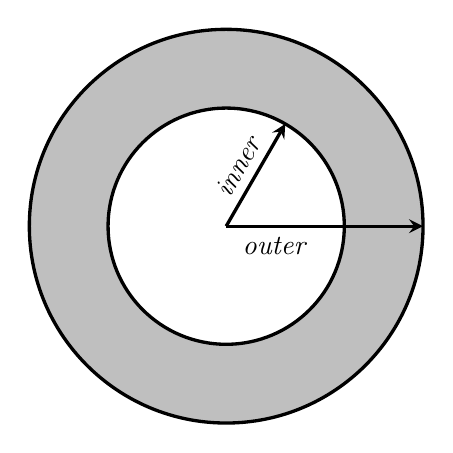
\begin{tikzpicture}[very thick,>=stealth]
      \filldraw[fill=lightgray,draw=black] (0,0) circle (25mm);
      \filldraw[fill=white,draw=black] (0,0) circle (15mm);
      \draw[->] (0,0) -- node[above,sloped]{$\mathit{inner}$} (60:15mm);
      \draw[->] (0,0) -- node[below,sloped,near start]{$\mathit{outer}$} (0:25mm);
    \end{tikzpicture}
  \end{center}

  \textbf{Vink:} brug funktionen \verb|circleArea| fra HR afsnit~1.2.
\item Erklær i en fil en funktion \verb|fooint : int * int -> int|,
  sådan at kaldet\newline \texttt{fooint($n$,$k$)} evaluerer til værdien $2n - k^2$ for heltal
  $n$ og $k$. Beregn \verb|fooint(3,2)|.

  Erklær dernæst en funktion \verb|fooreal : real * real -> real|,
  sådan at kaldet \texttt{fooreal($n$,$k$)} evaluerer til værdien $2n-k^2$
  for kommatal $n$ og $k$. Vær opmærksom på to-tallet. Beregn
  \verb|fooreal(3.0,2.0)|.

  Erklær dernæst en funktion \verb|foomix : real * int -> real|, sådan
  at kaldet \texttt{foomix($n$,$k$)} evaluerer til værdien $2n - k^2$ for
  kommatal $n$ og heltal $k$. Bemærk de forskellige typer af argumenterne
  til minus. Hvordan håndterer du det? Beregn \verb|foomix(3.0,2)|.

\item Omskriv funtionerne \texttt{fact} og \texttt{power}, så de
  bruger \texttt{if-then-else} i stedet for mønstergenkendelse.

\item Hvis der er tid tilovers, løs opgave 1.3, 1.4, 2.1, 2.2 i
  HR samt 4.1--4.6 i IP-2.
\end{enumerate}

%\newpage
\section{Gruppeaflevering}
\label{sec:gruppeaflevering}

Gruppeafleveringer laves i grupper på op til fire personer (typisk
jeres læsegrupper).

I uge 1 er gruppeafleveringen frivillig, men det anbefales at aflevere
den og få feedback. Besvarelsen afleveres i Absalon. Der afleveres en
fil pr. gruppe, men den skal angive alle deltageres fulde navne i
kommentarlinjer øverst i filen. Filens navn skal være af formen
\texttt{1G-\textit{initialer}.sml}, hvor initialer er erstattet af
gruppemedlemmernes initialer. Hvis f.eks. Bill~Gates, Linus~Torvalds,
Steve~Jobs og Gabe~Logan~Newell afleverer en opgave sammen, skal filen
hedde \texttt{1G-BG-LT-SJ-GLN.sml}. Brug gruppeafleveringsfunktionen i
Absalon.  Ved genaflevering bruges samme navnekonvention, men med
``\texttt{-genafl}'' tilføjet før \texttt{.sml},
f.eks.\ \texttt{1G-BG-LT-SJ-GLN-genafl.sml}.  Lad filen fra den
oprindelige aflevering blive liggende.

I gymnasiet lærte I, at man kan løse andengradsligningen $ax^2 + bx +
c = 0$ med formlen
\[x = \frac{-b \pm \sqrt{b^2 - 4ac}}{2a}\]

Som giver 2 reelle løsninger, hvis $b^2 - 4ac \ge 0$ og ingen reelle
løsninger, hvis $b^2 - 4ac < 0$.

\begin{enumerate}[{1}G1]
\item Skriv en funtion %
  \verb|solve2 : real * real * real -> real * real|, sådan at\newline
  \verb|solve2 a b c| giver de to løsninger for $x$ i
  ligningen $ax^2 + bx + c = 0$, såfremt $b^2 - 4ac \ge 0$. Du behøver
  ikke tage stilling til tilfældet $b^2 - 4ac < 0$.  Vink:
  Kvadratrodsfunktionen hedder \verb|sqrt|.
\item Hvad giver kaldet \verb|solve2 2.0 3.0 1.0|? Er svaret rigtigt?
\item Hvad giver kaldet \verb|solve2 2.0 3.0 4.0|? Hvorfor?

\item Den potensfunktion \verb|power|, der er defineret i tirsdagsopgaverne
skal bruge 21 multiplikationer til at beregne \verb|power 2 21 |--helt
generelt bruges $n$ multiplikationer til at beregne
\verb|power a n|. Det kan gøres med væsentligt færre
multiplikationer ved at benytte regnereglen $a^{2n} = (a^n)^2$, når
man har en lige potens.

Skriv en ny potensfunktion \verb|powerNew : int * int -> int|, som
bruger denne regneregel til at reducere antallet af multiplikationer,
så f.eks. \verb|powerNew 2 21| kan beregnes med højest 11
multiplikationer. Vink: Brug funktionerne \verb|div| og \verb|mod|.

\item Udvid funktionen, så den udover $a^n$ også returnerer antallet
  af brugte multiplikationer. Lav altså en funktion %
  \verb|powerCount : int * int -> int * int|, sådan at
  \verb|powerCount a n| returnerer parret \texttt{($a^n$,$m$)},
  hvor $m$ er antallet af brugte multiplikationer. Vis resultatet for
  \verb|powerCount 2 21|.
\end{enumerate}

%\newpage
\section{Individuel aflevering}
\label{sec:indiv-aflev}

Også den individuelle opgave er frivillig i uge 1, men vi anbefaler
igen, at den afleveres. Den afleveres i Absalon som en fil med navnet
\texttt{1I-\textit{navn}.sml}, hvor \texttt{\textit{navn}} er
erstatttet med dit navn. Hvis du fx hedder Anders~A.~And, skal
filnavnet være \texttt{1I-Anders-A-And.sml}. Skriv også dit fulde navn
som en kommentar i starten af filen.  Ved genaflevering bruges samme
navnekonvention, men med ``\texttt{-genafl}'' tilføjet før
\texttt{.sml}, f.eks.\ \texttt{1I-Anders-A-And-genafl.sml}.  Lad filen
fra den oprindelige aflevering blive liggende.

\begin{enumerate}[{1I}1]
\item Skriv en funktion \verb|powerRealInt: real * int -> real|,
  der givet et kommatal $a$ og et heltal $n$ beregner $a^n$. Funktionen
  skal virke både for positive og negative værdier af $n$. Brug reglen
  $a^{-n} = \frac{1}{a^n}$. Vis værdien af kaldet %
  \verb|powerRealInt 0.99 -100|.

\item Håndkør funktionen:

\begin{verbatim}
let rec mystisk m n =
    if (m = 0) then n 
    elif (m > n) then (mystisk (m-n) n)
    elif (m < n) then (mystisk m (n-m))
    else m
\end{verbatim}

med argumentet \verb|(21,56)| i samme stil som HR afsnit 2.4.
Vis håndkøringen i en kommentar i din afleverede .sml fil. Hvad beregner funktionen?

\item Definer en funktion \verb|rightAlign: int * int -> string|,
  sådan at kaldet\newline \texttt{rightAlign($n$,$w$)} returnerer en
  tekst af længde $w$, der indeholder tekstrepræsentationen af tallet
  $n$ højrestillet i teksten.  For eksempel skal
  \texttt{rightAlign(17,4)} returnere teksten \texttt{"{}~~17"} (som
  har længden 4).  Hvis der er mere end $w$ cifre i $n$, skal teksten
  indeholde alle cifrene (og evt.\ fortegn), selv om længden dermed
  overstiger $w$.  For eksempel skal \verb|rightAlign(~17,2)|
  returnere teksten \verb|"~17"| (som har længden 3).

\end{enumerate}

%\newpage
\section{Ugens nød}
\label{sec:ugens-nod}

\textbf{>>[Rework needed]: Der mangle parameter angivelser. Det kan betyde endeløst mange forskellige ting}
Ugens nød er en frivillig, særligt udfordrende opgave, der kan løses
af særligt interesserede studerende.  Opgaven kan løses kun ved brug
af begreber, der allerede er undervist i, men kræver ekstra omtanke og
nogen gange en god ide.  Afleveringsfristen er den samme som for den
individuelle opgave.  Ved fredagsforelæsningen i den efterfølgende uge
kåres den bedste løsning til ugens nød, og vinderen får en lille
præmie, typisk et stykke chokolade eller andet guf.

\begin{center}
\scalebox{0.8}{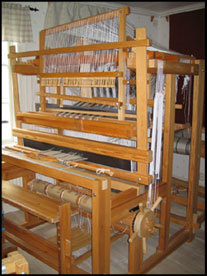
\includegraphics{uge1_vaev.jpg}}
\end{center}

På en gammeldags pedalvæv (som den herover viste) laves mønstre i
stoffet ved, at trendtråde og skudtråde er over eller under hinanden.
Dette sker ved, at man med pedaler kan løfte eller sænke trendtrådene,
så skyttelen (der leder skudtråden igennem) kommer under de løftede
tråde men over de sænkede.  Ved i forskellige rækker at løfte/sænke
forskellige tråde, laves forskellige mønstre.  I lærredsvævning løfter
man f.eks.\ på skift de lige og de ulige tråde, så der opstår et
``skakbræt'' mønster.

Vi antager, at der er fire pedaler nummereret 1 til 4.  Hver pedals
opførsel beskrives som et $m$-cifret tal ($2\leq m\leq 8$) med cifrene
1 og 2, hvor 1 betyder ``sænk'' og 2 betyder ``løft''.  De $m$ første
trendtråde vil blive løftet og sænket efter denne opskrift, hvorefter
mønstret gentages for de næste $m$ tråde osv. hele vejen gennem alle
trendtråde.

Rækkefølgen af trædning på pedaler ved hvert skyttelskud giver
mønstret. Denne rækkefølge beskrives som et $n$-cifret tal ($2\leq
n\leq 8$), hvor cifrene er 1 til 4, svarene til pedalernes numre.

For eksempel vil pedalerne for lærredsvævning beskrives med tallene
12, 21 og to vilkårlige tal (som vi ikke bruger), og pedalrækkefølgen
som 12, idet man skifter mellem de to pedaler.

Pepitatern (nummer 2 herunder):

\begin{center}
\scalebox{0.8}{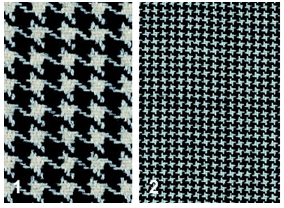
\includegraphics{uge1_pepita.png}}
\end{center}

laves med følgende fire pedaler:

\begin{tabular}{rr}
1: & 1211\\
2: & 2111\\
3: & 2221\\
4: & 2212
\end{tabular}

som gentages i rækkefølgen 1234.  Det antages at trendtråde er hvide
og skudtråde er sorte.

\begin{enumerate}[{1}N1]

\item Skriv en funktion

\texttt{vaev : int * int * int * int * int * int * int -> string}

som givet tal for $m$, de fire pedaler, $n$ og pedalrækkefølgen
returnerer en tekst, der viser mønstret ved at vise \texttt{+} for
hvide tråde og \texttt{\#} for sorte tråde.

For eksempel skal kaldet \texttt{vaev (4, 1211, 2111, 2221, 2212, 4,
  1234)} returnere teksten \verb|"+#++\n#+++\n###+\n##+#\n"|, sådan at
hvis man skriver

\texttt{print(vaev (4, 1211, 2111, 2221, 2212, 4, 1234))}

får man vist teksten

\begin{Verbatim}[baselinestretch=0.8]
+#++
#+++
###+
##+#
\end{Verbatim}

\item Det kan være svært at få et indtryk af mønstret uden at se en
  gentagelse af det.  Skriv derfor en funktion

\texttt{vaev2 : int * int * int * int * int * int * int  * int -> string}

der givet de samme parametre som før samt et heltal $k$ viser mønstret
gentaget $k$ gange både vandret og lodret.  For eksempel skal kaldet


\texttt{print(vaev2 (4, 1211, 2111, 2221, 2212, 4, 1234, 3))}

vise teksten

\begin{Verbatim}[baselinestretch=0.8]
+#+++#+++#++
#+++#+++#+++
###+###+###+
##+###+###+#
+#+++#+++#++
#+++#+++#+++
###+###+###+
##+###+###+#
+#+++#+++#++
#+++#+++#+++
###+###+###+
##+###+###+#
\end{Verbatim}

\end{enumerate}

\end{document}

%%% Local Variables:
%%% mode: latex
%%% TeX-master: t
%%% End:
